\documentclass[tikz,border=10pt]{standalone}
\usepackage{amsmath,amssymb}
\usepackage{tikz}
\usetikzlibrary{arrows.meta,calc,patterns,positioning,shapes,decorations.markings,backgrounds,fit}

% Atlas colors
\definecolor{AtlasTeal}{HTML}{5BA4A4}
\definecolor{AtlasTealDark}{HTML}{4A8F8F}
\definecolor{AtlasTealLight}{HTML}{E8F4F4}
\definecolor{AtlasDeep}{HTML}{2C5F5F}
\definecolor{AtlasSage}{HTML}{7BAE7F}
\definecolor{AtlasSageLight}{HTML}{EDF5EE}
\definecolor{AtlasWarm}{HTML}{D4A853}
\definecolor{AtlasWarmLight}{HTML}{FDF6E8}

\begin{document}
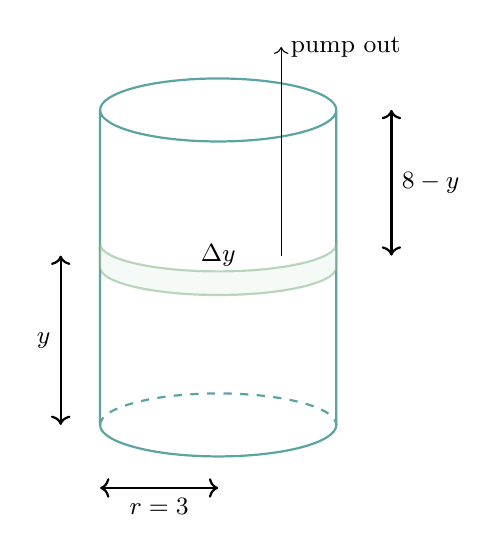
\begin{tikzpicture}
  % Cylindrical tank diagram
  \draw[AtlasTeal, thick] (-1.5,0) -- (-1.5,4) arc (180:360:1.5 and 0.4) -- (1.5,0);
  \draw[AtlasTeal, thick] (-1.5,0) arc (180:360:1.5 and 0.4);
  \draw[AtlasTeal, thick, dashed] (-1.5,0) arc (180:0:1.5 and 0.4);
  \draw[AtlasTeal, thick] (-1.5,4) arc (180:0:1.5 and 0.4);
  
  % Water layer
  \draw[AtlasSage, thick, fill=AtlasSageLight, opacity=0.5] 
    (-1.5,2) arc (180:360:1.5 and 0.35) -- (1.5,2.3) arc (360:180:1.5 and 0.35) -- cycle;
  
  % Annotations
  \draw[<->, thick] (-2,0) -- node[left, font=\small] {$y$} (-2,2.15);
  \draw[<->, thick] (2.2,2.15) -- node[right, font=\small] {$8-y$} (2.2,4);
  \draw[<->, thick] (-1.5,-0.8) -- node[below, font=\small] {$r=3$} (0,-0.8);
  
  \node[font=\small] at (0,2.15) {$\Delta y$};
  \draw[->] (0.8,2.15) -- (0.8,4.8) node[right, font=\small] {pump out};
\end{tikzpicture}
\end{document}
